\documentclass[dvisvgm,multi=true]{standalone}
\usepackage{mathmlcoresvg}
\begin{document}

% <figcaption><span>Figure 2: </span>Examples of italic correction for italic f and large integral</figcaption>
  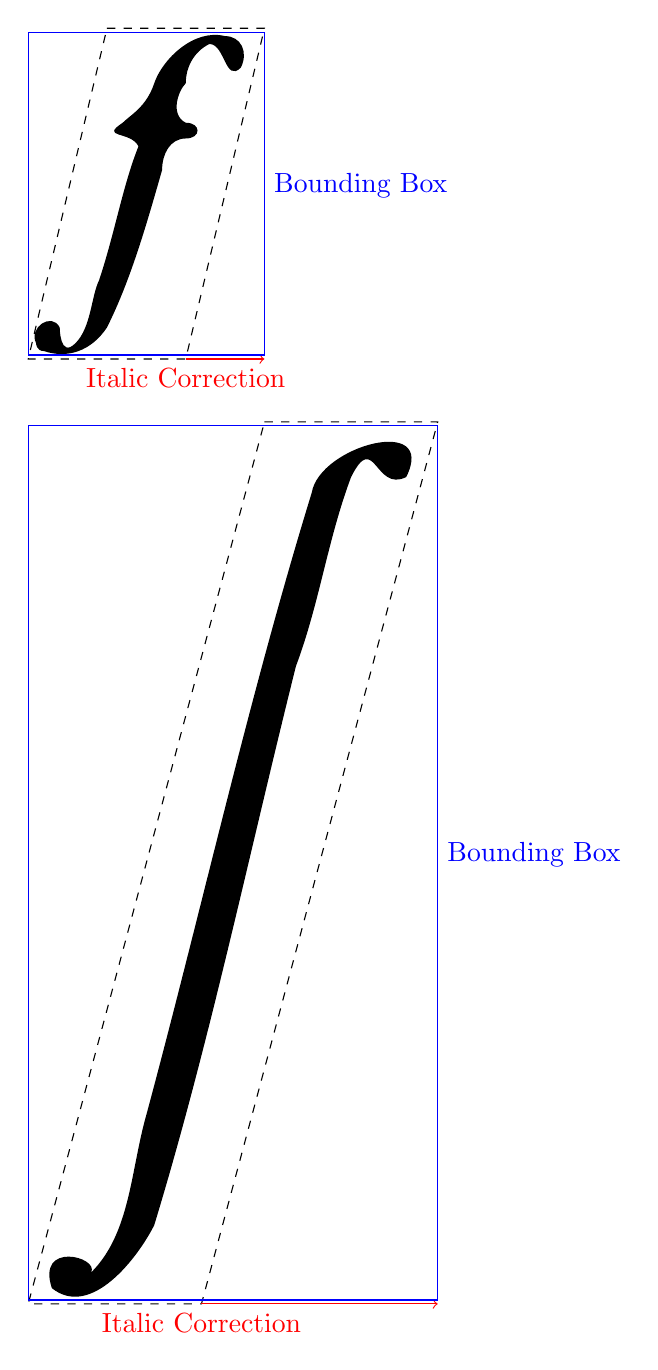
\begin{tikzpicture}[yscale=-1]

    \begin{scope}[xscale=.1,yscale=.1]
    \fill[black] (1,40) .. controls (0,38) and (3,36) .. (4,38) .. controls (4,38) and (4,42) .. (6,40) .. controls (8,38) and (8,34) .. (9,32) .. controls (11,26) and (12,20) .. (14,15) .. controls (13,13) and (9,14) .. (12,12) .. controls (13,11) and (15,10) .. (16,7) .. controls (17,4) and (21,0) .. (25,1) .. controls (27,1) and (28,3) .. (27,5) .. controls (25,7) and (25,2) .. (23,2) .. controls (21,3) and (20,5) .. (20,7) .. controls (19,8) and (18,11) .. (20,12) .. controls (22,12) and (22,14) .. (20,14) .. controls (18,14) and (17,16) .. (17,18) .. controls (15,25) and (13,32) .. (10,38) .. controls (8,41) and (5,42) .. (2,41) .. controls (1,41) and (1,40) .. (1,40) -- cycle;
    \draw[black,dashed] (10,0) -- (30,0) -- (20,42) -- (0,42) -- cycle;
    \draw[red,->] (20,42) node[below]{Italic Correction} -- (30,42);
    \draw[blue] (0,.5) -- (30,.5) --
    (30,20) node[right]{Bounding Box} --
    (30,41.5) -- (0,41.5) -- cycle;
    \end{scope}

    \begin{scope}[shift={(0,5)},xscale=.1,yscale=.1]
    \fill[black] (3,110) .. controls (1,104) and (9,106) .. (8,108) .. controls (13,103) and (13,95) .. (15,88) .. controls (22,62) and (28,35) .. (36,9) .. controls (37,3) and (52,-1) .. (48,7) .. controls (44,9) and (44,1) .. (41,7) .. controls (38,15) and (37,23) .. (34,31) .. controls (28,55) and (23,79) .. (16,102) .. controls (14,106) and (8,114) .. (3,110) -- cycle;
    \draw[black,dashed] (30,0) -- (52,0) -- (22,112) -- (0,112) -- cycle;
    \draw[red,->] (22,112) node[below]{Italic Correction} -- (52,112);

    \draw[blue] (0,.5) -- (52,.5) --
    (52,55) node[right]{Bounding Box} --
    (52,111.5) -- (0,111.5) -- cycle;

    \end{scope}
\end{tikzpicture}

\end{document}
